\clearpage
\setcounter{page}{1}
\maketitlesupplementary


% \section{Rationale}
% \label{sec:rationale}
% % 
% Having the supplementary compiled together with the main paper means that:
% % 
% \begin{itemize}
% \item The supplementary can back-reference sections of the main paper, for example, we can refer to \cref{sec:intro};
% \item The main paper can forward reference sub-sections within the supplementary explicitly (e.g. referring to a particular experiment); 
% \item When submitted to arXiv, the supplementary will already included at the end of the paper.
% \end{itemize}
% % 
% To split the supplementary pages from the main paper, you can use \href{https://support.apple.com/en-ca/guide/preview/prvw11793/mac#:~:text=Delete%20a%20page%20from%20a,or%20choose%20Edit%20%3E%20Delete).}{Preview (on macOS)}, \href{https://www.adobe.com/acrobat/how-to/delete-pages-from-pdf.html#:~:text=Choose%20%E2%80%9CTools%E2%80%9D%20%3E%20%E2%80%9COrganize,or%20pages%20from%20the%20file.}{Adobe Acrobat} (on all OSs), as well as \href{https://superuser.com/questions/517986/is-it-possible-to-delete-some-pages-of-a-pdf-document}{command line tools}.

\section*{A. Overall Training Procedure}
We summarize the complete optimization process of our framework in Algorithm~\ref{alg:CUE}.
It outlines how the baseline logit-adjusted loss and the two binary logit-adjusted terms 
are jointly optimized within each minibatch.

\begin{algorithm}[h]
\SetCustomAlgoRuledWidth{0.45\textwidth}
\SetAlgoLined
\caption{\textbf{CUE:Concept-Aware Multi-Label Expansion}}
\label{alg:CUE}
\KwIn{Training set $\mathcal{D}=\{(x_i,y_i)\}$, class prior $\pi_c$, CLIP model $\theta^{\text{zs}}$, LLM prior $\mathcal{N}^{\text{llm}}$}
\KwOut{Optimized model parameters $\Theta$}

\For{each minibatch $(\mathbf{x}_i, y_i)$}{
     Compute logits by model: $\theta(\mathbf{x}_i)=f(\mathbf{x}_i;\Theta)$ \\[4pt]
    
    Compute $\mathcal{L}^{\text{LA}}$ by Eq.~(5). \\[4pt]
    
    \textbf{VLM prior:} $\tilde{\mathbf{t}}^{\text{zs}}_i = \mathbf{1}_{\{c \in \{y_i\}\cup \text{Top-}k(\theta^{\text{zs}}(\mathbf{x}_i))\}}$ \\[4pt]
    
     \textbf{LLM prior:} $\tilde{\mathbf{t}}^{\text{llm}}_i = \mathbf{1}_{\{c \in \{y_i\}\cup \mathcal{N}^{\text{llm}}(y_i)\}}$ \\[4pt]
    
     Compute $\mathcal{L}^{\text{BLA}}_{\text{VLM}}$ and $\mathcal{L}^{\text{BLA}}_{\text{LLM}}$ by Eq.~(6). \\[4pt]
    
    \textbf{Joint optimization:} Combine all terms:
    \[
    \mathcal{L} = \mathcal{L}^{\text{LA}} 
    + \lambda_{\text{zs}}\mathcal{L}^{\text{BLA}}_{\text{VLM}} 
    + \lambda_{\text{llm}}\mathcal{L}^{\text{BLA}}_{\text{LLM}}
    \] \\[4pt]
    
     Update $\Theta \leftarrow \Theta - \eta \nabla_\Theta \mathcal{L}$
}


\end{algorithm}

\section*{B. Proof of Logit Adjustment Formulation}
\subsection*{B.1. Proof of LA}

Consider a long-tailed training distribution
\[
P_{\text{train}}(x,y), \qquad P_{\text{train}}(y=c)=\pi_c,
\]
where $\pi_c$ is the empirical class prior.  
Under the training prior, Bayes' rule gives
\[
P_{\text{train}}(y=c \mid x)
\propto P(x \mid y=c)\,\pi_c,
\]
while under the desired balanced prior
\[
P_{\text{bal}}(y=c)=\frac{1}{C},
\qquad
P_{\text{bal}}(y=c \mid x)
\propto P(x \mid y=c)\,\frac{1}{C}.
\]
Dividing the two posteriors yields
\[
P_{\text{bal}}(y=c \mid x)
\propto
\frac{P_{\text{train}}(y=c \mid x)}{\pi_c}.
\]
Assume the model outputs logits $\theta_c(x)$ such that
\[
P_{\text{train}}(y=c \mid x)
=
\frac{\exp(\theta_c(x))}{\sum_j \exp(\theta_j(x))}
=
\text{softmax}_c(\theta(x)),
\]
we obtain the balanced-posterior form
\[
\begin{aligned}
P_{\text{bal}}(y=c \mid x)
&= \frac{\exp(\theta_c(x)-\log\pi_c)}
        {\sum_k \exp(\theta_k(x)-\log\pi_k)} \\
&= \text{softmax}_c\!\big(\theta_c(x)-\log\pi_c\big).
\end{aligned}
\]
Thus we define logit-adjusted logits
\[
\theta'_c(x)=\theta_c(x)+\tau\log\pi_c,
\]
where $\tau$ is a temperature coefficient: $\tau<0$ is used during training, while $\tau>0$ is used as a post-hoc adjustment during testing. Applying cross-entropy on $\theta'(x)$ yields the LA loss in Eq.~(5).

\subsection*{B.2. Proof of BLA}
For the multi-label setting, each class $c$ is associated with a binary
variable $z_c\in\{0,1\}$, with
\[
P_{\text{train}}(z_c=1)=P_{\text{train}}(y=c)=\pi_c,
\]
and the balanced prior
\[
P_{\text{bal}}(z_c=1)=\frac{1}{C}.
\]
Analogous to the multiclass case, Bayes' rule gives the posterior relation
\[
P_{\text{bal}}(z_c=1 \mid x).
\]
Assuming the model outputs logits $\theta_c(x)$ such that
\[
P_{\text{train}}(z_c=1\mid x)=\sigma(\theta_c(x)),
\]
we obtain the \emph{exact} balanced posterior logit:
\[
\begin{aligned}
\theta_c^{\text{bal}}(x)
&:= \log\frac{P_{\text{bal}}(z_c=1\mid x)}{P_{\text{bal}}(z_c=0\mid x)}  \\
&= \theta_c(x)
+ \log\frac{\frac{1}{C}}{\frac{C-1}{C}}
- \log\frac{\pi_c}{1-\pi_c} \\
&= \theta_c(x)
+ \log\frac{1}{C-1}
- \log\frac{\pi_c}{1-\pi_c}.
\end{aligned}
\]
In long-tailed learning settings, $C$ is typically fixed. Under this regime, the balanced logit reduces to the
following long-tailed approximation:
\[
\theta_c^{\text{bal}}(x)
\approx 
\theta_c(x) - \log\pi_c + \log(1-\pi_c) + \text{const},
\]
where the constant term is class-independent and thus does not affect class-wise relative preference. At this point, the balanced logit for the binary case can already be used directly for training. 
However, noting that the term $-\log\pi_c$ is the dominant class-dependent factor under long-tailed 
priors, and in order to maintain consistency with the multiclass LA formulation (thus simplifying 
implementation), we adopt the same prior-adjustment form as LA:
\[
\tilde\theta_c(x)=\theta_c(x)+\tau_b\log\pi_c,
\]
where $\tau_b$ is a temperature coefficient (typically $\tau_b<0$ during training). Applying binary
cross-entropy to $\tilde\theta_c(x)$ with multi-label targets $\tilde t_{i,c}$ yields the BLA loss in
Eq.~(6).



\section*{C. Additional Results on Different Top-$k$ Settings}
In addition to the main results reported in the paper, we further evaluate the 
effect of different Top-$k$ selections used in constructing VLM-based instance 
cues. Experiments are conducted on both ImageNet-LT and Places-LT, with 
$k \in \{10, 20, 50\}$. The results in Table~\ref{tab:topk_all} show that CUE 
remains consistently stable across different $k$ values on both benchmarks.
% Experiments conducted on Places-LT and ImageNet-LT
\begin{table}[h]
\centering
\caption{Results under different Top-$k$ settings. We report All / Many / Medium / Few performance.}
\label{tab:topk_all}
\small
\begin{tabular}{l|cccc}
\toprule
\textbf{Top-k} & \textbf{All} & \textbf{Many} & \textbf{Med.} & \textbf{Few} \\
\midrule
\textcolor{gray}{\textbf{ImageNet-LT}} & & & & \\
\quad Top-10 & \textbf{77.5} & \textbf{80.3} & 76.4 & 73.4 \\
\quad Top-20 & \textbf{77.5} & 80.2 & 76.3 & \textbf{73.6} \\
\quad Top-50 & \textbf{77.5} & 80.2 & \textbf{76.5} & 73.2 \\[3pt]
\midrule
\textcolor{gray}{\textbf{Places-LT}} & & & & \\
\quad Top-10 & \textbf{51.7} & 50.6 &	\textbf{52.2} & 52.4 \\
\quad Top-20 &51.6& 50.6&	52.1	&\textbf{52.5}	 \\
\quad Top-50 & 51.6 & \textbf{50.9}	&\textbf{52.2}	&  51.4	 \\
\bottomrule
\end{tabular}
\vspace{-1em}
\end{table}


\section*{D. Extension to Additional Benchmarks}
% Expanded evaluations on Places-LT and ImageNet-LT
To further assess the generality of CUE beyond the benchmarks reported in the 
main paper, we extend our evaluation to Places-LT and ImageNet-LT. We conduct experiments using both PEFT-based adaptation methods and from-scratch training baselines, As shown in the 
following sections.

\subsection*{D.1 Results on Places-LT}
 As shown in Table~\ref{tab:places_peft_scratch}, CUE consistently brings improvements across different adaptation paradigms, especially on the Few-shot categories. For the from-scratch setting, following prior work\cite{kang2020decoupling,cui2022reslt}, we adopt a ResNet-152 backbone initialized from an ImageNet-pretrained checkpoint and train the model for 30 epochs using a cosine learning rate schedule from 0.1 to 0.

\begin{table}[h]
\centering
\caption{Results on Places-LT using PEFT methods and from-scratch baselines. 
We report All / Many / Med. / Few performance.}
\label{tab:places_peft_scratch}
\small
\begin{tabular}{l|cccc}
\toprule
\textbf{Method} & \textbf{All} & \textbf{Many} & \textbf{Med.} & \textbf{Few} \\
\midrule
\textcolor{gray}{\textbf{PEFT}} & & & & \\
\quad 
LoRA~\cite{hu2022lora} &51.0 & \textbf{50.5}	&\textbf{51.9}	&50.0	  \\
\quad + CUE & \textbf{51.1} & 50.4	&51.7	&\textbf{50.8}	\\
\quad VPT-shallow~\cite{jia2022visual} & 49.2 & \textbf{49.5} &	\textbf{51.0}	& 44.6	  \\
\quad + CUE & \textbf{49.2} & 48.5 &	50.8 & \textbf{46.9}  \\
\quad VPT-deep~\cite{jia2022visual} & 50.9 & \textbf{50.8}	& \textbf{51.8} &49.0	  \\
\quad + CUE & \textbf{50.9} &50.7	&51.3	&\textbf{50.3}	  \\
\quad 
Adapter~\cite{houlsby2019parameter} & 51.3& \textbf{51.1}&	\textbf{52.0}&	50.0	 \\
\quad + CUE & \textbf{51.3} & 50.5 &	51.8	& \textbf{51.6}	 \\[3pt]
\midrule
\textcolor{gray}{\textbf{From Scratch}} & & & & \\
\quad LA~\cite{menon2021longtail} & 37.0 & 42.0 & 36.9 & 28.7 \\
\textbf{}\quad + CUE & \textbf{37.3}  & \textbf{42.0}  & \textbf{37.0} & \textbf{30.0} \\
\quad ResLT~\cite{cui2022reslt} & 35.6 & \textbf{34.6} & 39.3 & 30.0 \\
\quad + CUE & \textbf{36.6}  & 32.4 & \textbf{40.8} & \textbf{35.0} \\
\bottomrule
\end{tabular}
\vspace{-1em}
\end{table}



\subsection*{D.2 Results on ImageNet-LT}
We further evaluate CUE on ImageNet-LT to examine its effectiveness across 
different settings. As shown in Table~\ref{tab:imagenet_peft_scratch}, 
CUE consistently improves performance for both PEFT-based methods and 
from-scratch baselines, with clear gains on medium- and few-shot categories.
For the from-scratch experiments, we follow the standard ImageNet-LT protocol 
and train a ResNet-50 backbone for 90 epochs using SGD. The learning rate is 
initialized at 0.1 and annealed to 0 using a cosine decay schedule.
\begin{table}[h]
\centering
\caption{Results on ImageNet-LT using PEFT methods and from-scratch baselines. 
We report All / Many / Med. / Few performance.}
\label{tab:imagenet_peft_scratch}
\small
\begin{tabular}{l|cccc}
\toprule
\textbf{Method} & \textbf{All} & \textbf{Many} & \textbf{Med.} & \textbf{Few} \\
\midrule
\textcolor{gray}{\textbf{PEFT}} & & & & \\
\quad 
LoRA~\cite{hu2022lora}  & 75.8 & 78.7	& 75.2 &	70.0 \\
\quad + CUE	&\textbf{76.3} & \textbf{78.9} & \textbf{75.7} & \textbf{70.9}\\
\quad VPT-shallow~\cite{jia2022visual} &  74.2  & \textbf{77.9} & 73.9 & 65.3 
\\
\quad + CUE & \textbf{74.7} & 77.7 & \textbf{74.4} & \textbf{67.1}  \\
\quad VPT-deep~\cite{jia2022visual} & 76.1 & 78.6  & 75.4  & 71.2  \\
\quad + CUE & \textbf{76.3} & \textbf{78.8} & \textbf{75.7} & \textbf{71.8} \\
\quad Adapter~\cite{houlsby2019parameter} & 76.9 & \textbf{80.2} & 75.9 & 71.2 \\
\quad + CUE & \textbf{77.2} &  80.0 & \textbf{76.2} & \textbf{72.7} \\[3pt]
\midrule
\textcolor{gray}{\textbf{From Scratch}} & & & & \\
\quad LA~\cite{menon2021longtail} & 49.1 & \textbf{59.8}  & 46.6 & 28.9 \\
\quad + CUE &  \textbf{49.4} & 59.8 & \textbf{46.8} & \textbf{30.1} \\
\quad ResLT~\cite{cui2022reslt} & 46.9 & \textbf{52.2}& 47.3 & 31.4\\
\quad + CUE & \textbf{47.6} & 52.2  & \textbf{48.1} & \textbf{33.7} \\
\bottomrule
\end{tabular}
\vspace{-1em}
\end{table}


               
\section*{E. Multi-Label Mappings}
\subsection*{E.1. LLM-based Class-level Mappings} We provide examples of the expanded multi-label targets generated by the 
LLM prior. All semantic neighbors are obtained using the \textbf{Qwen-plus} model, 
queried with the prompt described in Section~F. The mappings below illustrate 
how concept-level similarity leads to meaningful auxiliary labels that enrich 
the supervision signal.

\begin{table}[h]
\centering
\small
\caption{Examples of LLM-based cues produced by \textbf{Qwen-plus}.}
\begin{tabular}{p{0.30\linewidth}|p{0.60\linewidth}}
\toprule
\textbf{Class} & \textbf{Expanded Cues} \\
\midrule
\texttt{apple} &
\texttt{[orange, pear, mushroom, sweet\_pepper]} \\
\texttt{aquarium\_fish} &
\texttt{[dolphin, shark, trout, ray, seal]} \\
\texttt{willow\_tree} &
\texttt{[maple\_tree, oak\_tree, pine\_tree, palm\_tree, forest]} \\
\texttt{woman} &
\texttt{[man, girl, boy, baby]} \\
\texttt{worm} &
\texttt{[snail, snake, spider, beetle, caterpillar ]} \\
\bottomrule
\end{tabular}
\end{table}

\subsection*{E.2. VLM-based Instance-level Mappings.}
We also visualize the instance-level expansions generated from the VLM prior. 
Each figure shows one input image along with the top-$5$ VLM cues used as 
additional labels.

\begin{figure}[h]
    \centering
    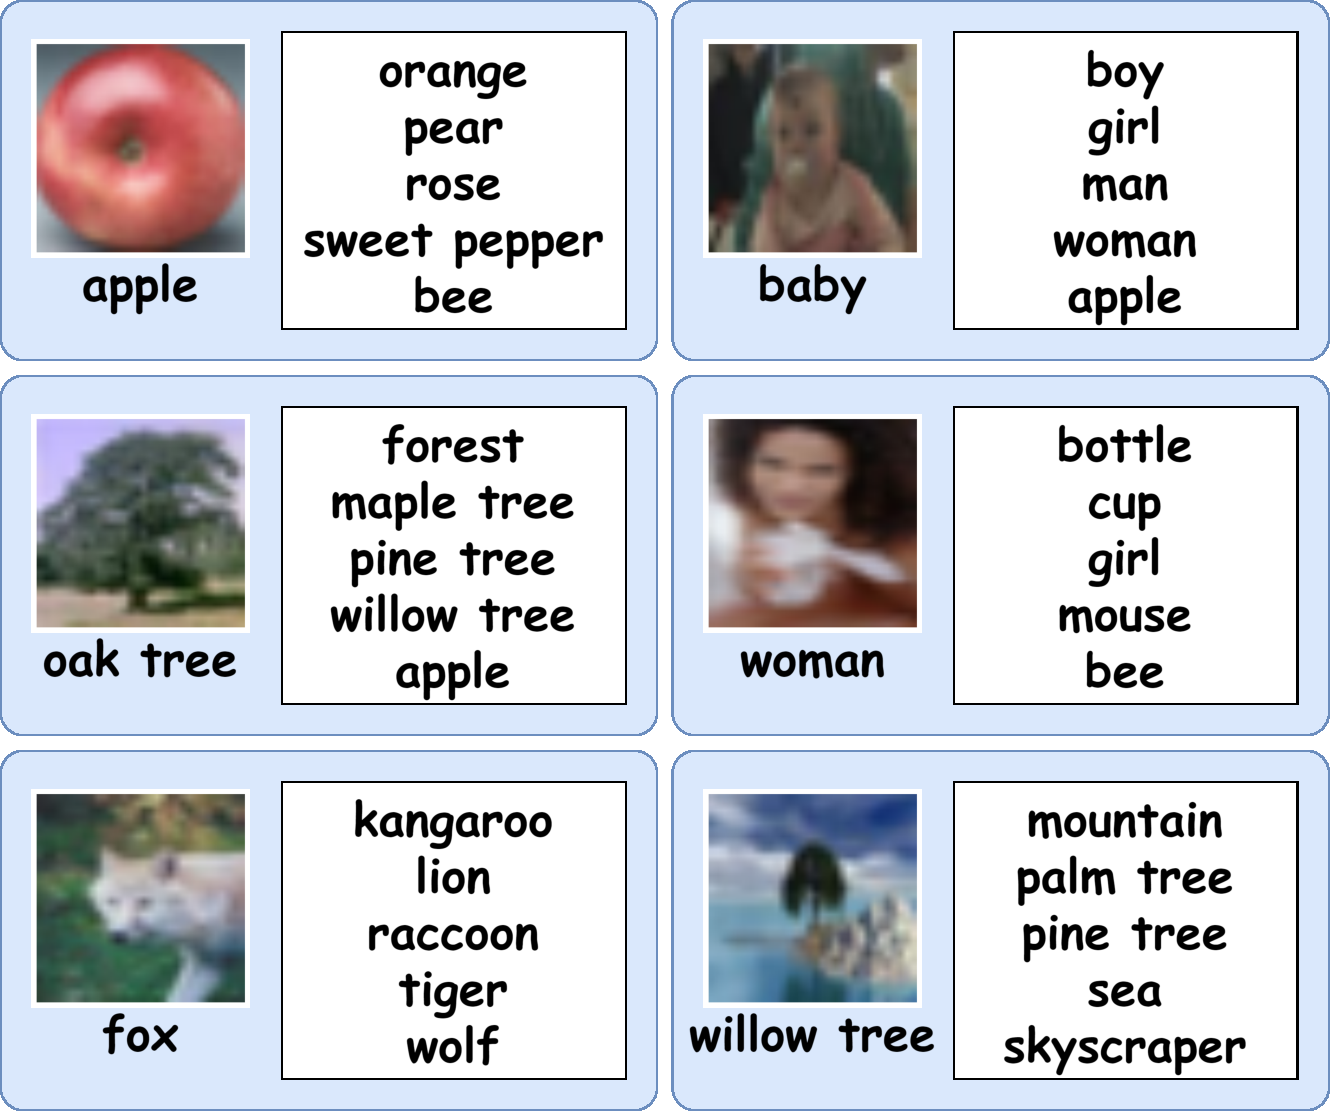
\includegraphics[width=1.0\linewidth]{img/vlm_mapping.pdf}
    \caption{Example VLM-based cues for the query images.}
    \label{fig:vlm_mapping_example}
\end{figure}

\section*{F. Prompts Used for Querying the LLM}

We use the following prompt template to obtain cues from the LLM.
The prompt is shown below. The red-highlighted placeholders will be dynamically replaced with real values.

\begin{quote}
\ttfamily
You are given a complete list of all\_classes: \colorbox{red!25}{\{all\_classes\}}

Task: Find similar classes for \colorbox{red!25}{\{batch\}}, using items from the 
complete list above.

Requirements:

- Return a valid JSON object only.

- Use the following format:
\{
  "class1": ["similar1", "similar2"],
  "class2": ["similar1", "similar2"]
\}

- Only choose from the provided complete list.

- Output JSON only, no additional explanation.
\end{quote}




\section*{G. Token Usage Statistics}
We report the total token usage incurred during the generation of LLM-based 
cues. For each dataset, class names are grouped into batches and queried using the prompt described in Section~F. Table~\ref{tab:token_cost} 
summarizes the approximate number of tokens used for each dataset.

\begin{table}[h]
\centering
\caption{Approximate token usage for LLM-based neighbor generation.}
\label{tab:token_cost}
\small
\begin{tabular}{l|c|c}
\toprule
\textbf{Dataset} & \textbf{\#Classes} & \textbf{Total Tokens} \\
\midrule
CIFAR100-LT  & 100  & $\sim$8.4K \\
Places-LT    & 365  & $\sim$85.6K \\
ImageNet-LT  & 1000 & $\sim$539.6K \\
iNaturalist  & 8142 & $\sim$57.3M \\
\bottomrule
\end{tabular}
\end{table}

All token costs remain inexpensive under modern LLM API pricing, and 
the process needs to be performed only once per dataset.
